\documentclass{scrreprt}

% Based on the template of Jean-Philippe Eisenbarth:
% - https://github.com/jpeisenbarth/SRS-Tex
% Based on the code of Yiannis Lazarides:
% - http://tex.stackexchange.com/questions/42602/software-requirements-specification-with-latex
% - http://tex.stackexchange.com/users/963/yiannis-lazarides
% Also based on the template of Karl E. Wiegers:
% - http://www.se.rit.edu/~emad/teaching/slides/srs_template_sep14.pdf
% - http://karlwiegers.com

\usepackage{listings}
\usepackage{underscore}
\usepackage[bookmarks=true]{hyperref}
\usepackage[utf8]{inputenc}
\usepackage[english]{babel}
\usepackage{hyperref}
\usepackage{wrapfig}
\usepackage{url}
\usepackage{enumitem}
\usepackage{graphicx}

\hypersetup{
    bookmarks=false,                                % show bookmarks bar?
    pdftitle={Software Requirement Specification},  % title
    pdfauthor={Jean-Philippe Eisenbarth},           % author
    pdfsubject={TeX and LaTeX},                     % subject of the document
    pdfkeywords={TeX, LaTeX, graphics, images},     % list of keywords
    colorlinks=true,                                % false: boxed links; true: colored links
    linkcolor=blue,                                 % color of internal links
    citecolor=black,                                % color of links to bibliography
    filecolor=black,                                % color of file links
    urlcolor=black,                                % color of external links
    linktoc=page                                    % only page is linked
}

\def\myversion{0.1.0 }
\def\projname{Ensemble Toolkit for Earth Sciences: Seismic Inversion}
\def\projauthors{$<$Authors$>$}
\def\entk{Ensemble Toolkit}
\date{}
\title{}

\begin{document}


% ----------------------------------------------------------------------------
% Cover
% ----------------------------------------------------------------------------
\begin{flushright}
    \rule{16cm}{5pt}\vskip1cm
    \begin{bfseries}
        \Huge{SOFTWARE REQUIREMENTS\\ SPECIFICATION}\\
        \vspace{1.9cm}
        for\\
        \vspace{1.9cm}
        \projname \\
        \vspace{1.9cm}
        \LARGE{Version \myversion approved}\\
        \vspace{1.9cm}
        Prepared by \projauthors\\
        \vspace{1.9cm}
        Princeton University and Rutgers University\\
        \vspace{1.9cm}
        \today\\
    \end{bfseries}
\end{flushright}

\tableofcontents


% ----------------------------------------------------------------------------
% Revision History
% ----------------------------------------------------------------------------
\chapter*{Revision History}

\begin{center}
    \begin{tabular}{|c|c|c|c|}
        \hline
	    Name & Date & Reason For Changes & Version\\
        \hline
	    1 & 16-04-2017 & Initial version & 0.1.0\\
        \hline
	    %31 & 32 & 33 & 34\\
        %\hline
    \end{tabular}
\end{center}


% ----------------------------------------------------------------------------
% Introduction
% ----------------------------------------------------------------------------
\chapter{Introduction}

\section{Purpose}
%$<$Identify the product whose software requirements are specified in this 
%document, including the revision or release number. Describe the scope of the 
%product that is covered by this SRS, particularly if this SRS describes only 
%part of the system or a single subsystem.$>$

The purpose of the document is to capture, in detail, the requirements of the "Seismic Inversion" track of the "Ensemble Toolkit for Earth Sciences" project. This document will include all the system requirements, interface, interactions and limitations of this track. . This document is primarily intended to be proposed to a customer for its approval
and a reference for developing the first version of the system.

\section{Document Conventions}
%$<$Describe any standards or typographical conventions that were followed when 
%writing this SRS, such as fonts or highlighting that have special significance.  
%For example, state whether priorities  for higher-level requirements are assumed 
%to be inherited by detailed requirements, or whether every requirement statement 
%is to have its own priority.$>$

The requested features are listed in section 4 and the non-functional requirements are listed in section 5. Each of these requirements have a priority from the set \{HIGH, MEDIUM, LOW\}. Based on the number of requirements and their priority, a timeline will be created with each requirement and its expected time-to-completion.

\section{Intended Audience and Reading Suggestions}
%$<$Describe the different types of reader that the document is intended for, 
%such as developers, project managers, marketing staff, users, testers, and 
%documentation writers. Describe what the rest of this SRS contains and how it is 
%organized. Suggest a sequence for reading the document, beginning with the 
%overview sections and proceeding through the sections that are most pertinent to 
%each reader type.$>$

The document is created and iterated by both the users and developers together. This document is intended for the developers and project manager to get a complete understanding of the requirements of the system as expected by the user.

An early usecase document is available at [1]. [2] presents the current status and overall goal of the seismic inversion application. [3] provides a quick introduction to the current capabilities of the Ensemble Toolkit.

\section{Project Scope}
%$<$Provide a short description of the software being specified and its purpose, 
%including relevant benefits, objectives, and goals. Relate the software to 
%corporate goals or business strategies. If a separate vision and scope document 
%is available, refer to it rather than duplicating its contents here.$>$

$<$This might be better suited for Princeton $>$.

The project has the following goals:

\begin{itemize}[noitemsep]
\item increase the ultimate resolving power of global inversions through more efficient use of resources
\item open new avenues of scientific research,in particular, anisotropic inversions
\item a package is to be developed and shared with the wider seismology community
\end{itemize}

\section{References}
%$<$List any other documents or Web addresses to which this SRS refers. These may 
%include user interface style guides, contracts, standards, system requirements 
%specifications, use case documents, or a vision and scope document. Provide 
%enough information so that the reader could access a copy of each reference, 
%including title, author, version number, date, and source or location.$>$

[1] \url{https://docs.google.com/document/d/1EjUKJxsNNISBwZ9IXERyiCAISKb25mEwjhyi1gePCDk/edit?usp=sharing}

[2] \url{https://github.com/radical-collaboration/hpc-workflows/blob/master/docs/presentations/20161026_ET_Seismo.pdf}

[3] \url{https://github.com/radical-collaboration/hpc-workflows/blob/master/docs/presentations/Ensemble\%20Toolkit\%20-\%20Quick\%20Overview.pdf}

[4] \url{http://seisflows.readthedocs.io/en/latest/}

[5] \url{https://bitbucket.org/mpbl/simpy}


% ----------------------------------------------------------------------------
% Overall Description
% ----------------------------------------------------------------------------
\chapter{Overall Description}

This chapter provides an overview of the system. It will describe the context of the system and why its development is deemed necessary. It will broadly list the functions the system is expected to perform along with its interaction with other systems as well as the user. This chapter will also describe the intended users and the system environment for the current version of the system. It will conclude with a list of assumptions and foreseen constraints.


\section{Product Perspective}
%$<$Describe the context and origin of the product being specified in this SRS.  
%For example, state whether this product is a follow-on member of a product 
%family, a replacement for certain existing systems, or a new, self-contained 
%product. If the SRS defines a component of a larger system, relate the 
%requirements of the larger system to the functionality of this software and 
%identify interfaces between the two. A simple diagram that shows the major 
%components of the overall system, subsystem interconnections, and external 
%interfaces can be helpful.$>$

The system will be designed to execute the seismic inversion workflow, as represented in Figure~\ref{fig:seismic_wflow}, at scale on HPCs, more specifically on DoE Titan machine. The various sequential and concurrent stages of the workflow and the associated data movement will be captured using the \entk API.

\begin{wrapfigure}{R}{0.41\textwidth}
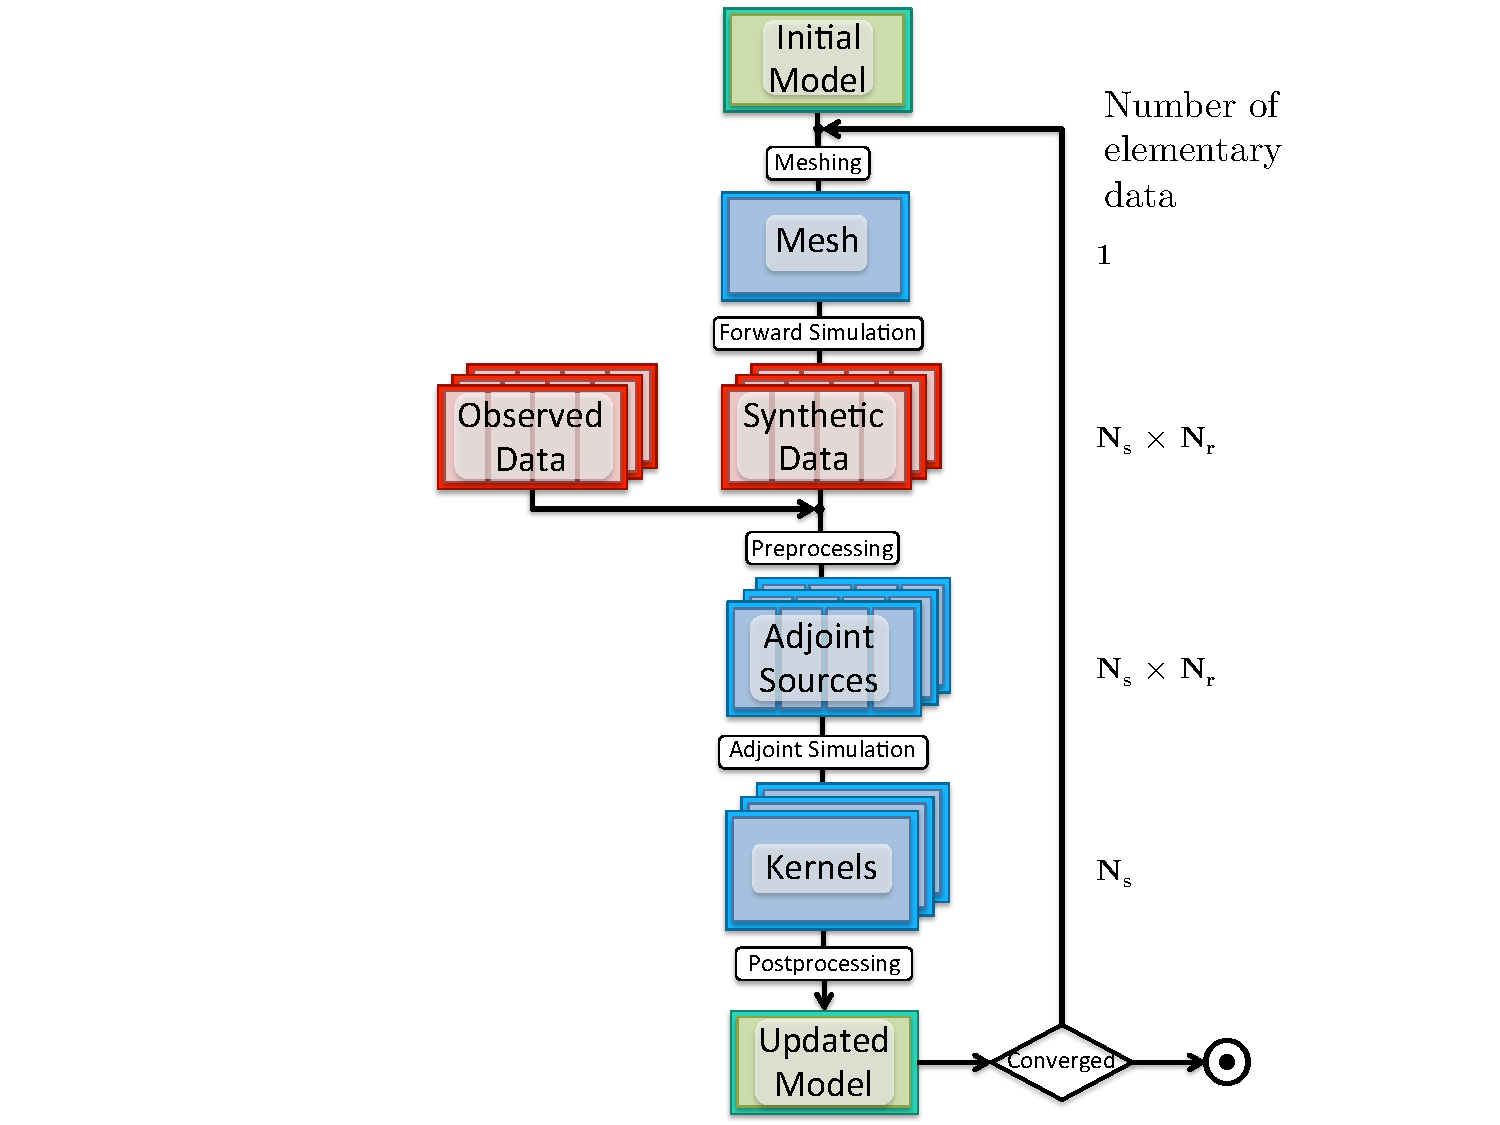
\includegraphics[width=0.4\textwidth]{SeismicWorkflow.pdf}
\caption{Seismic inversion workflow}
\label{fig:seismic_wflow}
\end{wrapfigure}

Existing solution executes the various stages of the workflow in parts: Seisflow[4] is the tool used to perform the simulations on an HPC and Simpy[5] is used to preprocess and postprocess the simulation data before the next set of simulations. This document captures the requirement of a product that will be an end-to-end solution addressing many of the missing features in the existing solution.

\begin{wrapfigure}{R}{0.41\textwidth}
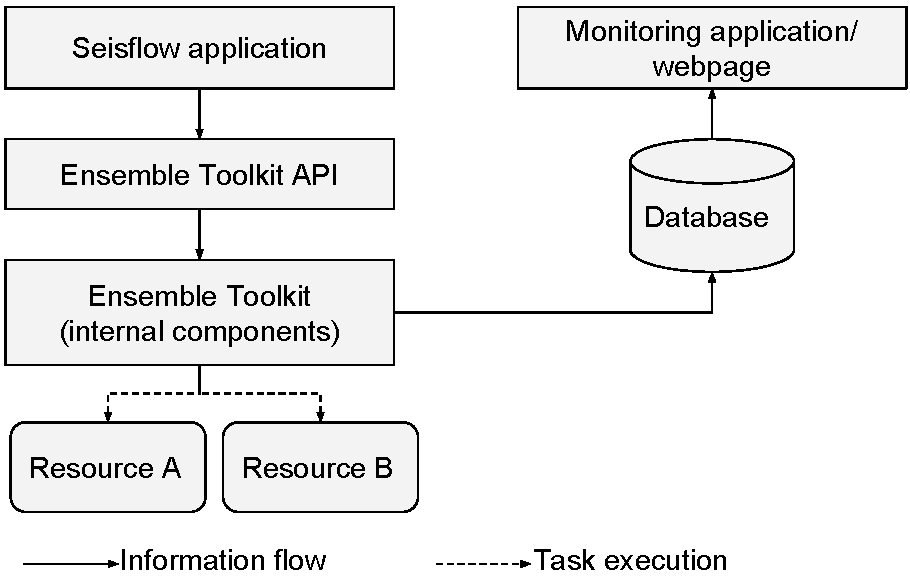
\includegraphics[width=0.4\textwidth]{seisflow-sys-design.pdf}
\caption{High-level design of the Ensemble Toolkit for Earth Sciences}
\label{fig:seisflow_sys_design}
\end{wrapfigure}

This system will be designed in order to expose, to the user, two components: an API and a database. The API will enable the user to describe the application workflow completely. The database will provide access to the state of the various tasks in the workflow. This will enable the user to observe performance metrics or perform various analysis in real time.
Once the application is described via the API, the internal components will translate the application into executable units and manage their execution across multiple resources. Figure~\ref{fig:seisflow_sys_design} provides a graphical representation of the system.



\section{Product Functions}
%$<$Summarize the major functions the product must perform or must let the user 
%perform. Details will be provided in Section 3, so only a high level summary 
%(such as a bullet list) is needed here. Organize the functions to make them 
%understandable to any reader of the SRS. A picture of the major groups of 
%related requirements and how they relate, such as a top level data flow diagram 
%or object class diagram, is often effective.$>$

The major functions the product is expected to perform is the following:

\begin{itemize}[noitemsep]
\item an API sufficient to capture the description of the complete workflow
\item capacity to execute O(1000) tasks concurrently
\item ability to manage task failures due to several reasons
\item ability to provide real time execution statistics and user access to intermediate data
\end{itemize}



\section{User Classes and Characteristics}
%$<$Identify the various user classes that you anticipate will use this product.  
%User classes may be differentiated based on frequency of use, subset of product 
%functions used, technical expertise, security or privilege levels, educational 
%level, or experience. Describe the pertinent characteristics of each user class.  
%Certain requirements may pertain only to certain user classes. Distinguish the 
%most important user classes for this product from those who are less important 
%to satisfy.$>$

The \myversion version of the product is intended to be used only by the Princeton and Rutgers groups. Later versions will be developed and packaged to be distributed to a wider community.

\section{Operating Environment}
%$<$Describe the environment in which the software will operate, including the 
%hardware platform, operating system and versions, and any other software 
%components or applications with which it must peacefully coexist.$>$

The primary OS the product will be tested on is Linux with possible support of MacOS. The primary HPCs the product will be tested on is the ORNL Titan, ORNL Rhea and TACC Stampede.

\section{Design and Implementation Constraints}
%$<$Describe any items or issues that will limit the options available to the 
%developers. These might include: corporate or regulatory policies; hardware 
%limitations (timing requirements, memory requirements); interfaces to other 
%applications; specific technologies, tools, and databases to be used; parallel 
%operations; language requirements; communications protocols; security 
%considerations; design conventions or programming standards (for example, if the 
%customer’s organization will be responsible for maintaining the delivered 
%software).$>$

The entire framework, including the API exposed to the user, will be python based but will support any task kernel intended for a Linux OS.

The current version will be using RADICAL Pilot (RP) as a runtime system and will be constrained to the performance limitations of the same. <TBA: Relevant RP performance numbers/plots>.

The forward and adjoint simulations will use the SPECFEM tool, available at \url{http://specfem3d-globe.readthedocs.io/en/latest/}. The preprocessing and postprocessing will use the pypaw tool, available at \url{https://github.com/wjlei1990/pypaw}.

\section{User Documentation}
%$<$List the user documentation components (such as user manuals, on-line help, 
%and tutorials) that will be delivered along with the software. Identify any 
%known user documentation delivery formats or standards.$>$

All the relevant code will be available on Github. Ensemble Toolkit code will be available at \url{https://github.com/radical-cybertools/radical.ensemblemd}. User manual for Ensemble Toolkit will be made available in \url{http://radicalensemblemd.readthedocs.org/en/latest/}. The code for the end-to-end workflow will be available on Github and user manual on \url{www.readthedocs.org}. The exact URLs will be updated as the project matures.

\section{Assumptions and Dependencies}

$<$List any assumed factors (as opposed to known facts) that could affect the 
requirements stated in the SRS. These could include third-party or commercial 
components that you plan to use, issues around the development or operating 
environment, or constraints. The project could be affected if these assumptions 
are incorrect, are not shared, or change. Also identify any dependencies the 
project has on external factors, such as software components that you intend to 
reuse from another project, unless they are already documented elsewhere (for 
example, in the vision and scope document or the project plan).$>$

The following assumptions have been made:
\begin{itemize}[noitemsep]
\item Currently, the framework requires no interactivity. If a manual halt is necessary, this requires starting (as opposed to resuming) from the last checkpoint or backup.
\item GPU-only simulation is sufficient.
\end{itemize}

The framework will have a dependency on the following tools:

\begin{itemize}[noitemsep]
\item RADICAL Pilot
\item Specfem3D
\item pypaw (and its dependencies)
\end{itemize}
% ----------------------------------------------------------------------------
% Interface Requirements
% ----------------------------------------------------------------------------
\chapter{External Interface Requirements}

\section{User Interfaces}
%$<$Describe the logical characteristics of each interface between the software 
%product and the users. This may include sample screen images, any GUI standards 
%or product family style guides that are to be followed, screen layout 
%constraints, standard buttons and functions (e.g., help) that will appear on 
%every screen, keyboard shortcuts, error message display standards, and so on.  
%Define the software components for which a user interface is needed. Details of 
%the user interface design should be documented in a separate user interface 
%specification.$>$

TBD

\section{Hardware Interfaces}
%$<$Describe the logical and physical characteristics of each interface between 
%the software product and the hardware components of the system. This may include 
%the supported device types, the nature of the data and control interactions 
%between the software and the hardware, and communication protocols to be 
%used.$>$

The interaction between the product and the hardware, both on the local and remote ends, is abstracted from the user. The hardware interaction is complex and can be deemed out of scope for the current document.

\section{Software Interfaces}
%$<$Describe the connections between this product and other specific software 
%components (name and version), including databases, operating systems, tools, 
%libraries, and integrated commercial components. Identify the data items or 
%messages coming into the system and going out and describe the purpose of each.  
%Describe the services needed and the nature of communications. Refer to 
%documents that describe detailed application programming interface protocols.  
%Identify data that will be shared across software components. If the data 
%sharing mechanism must be implemented in a specific way (for example, use of a 
%global data area in a multitasking operating system), specify this as an 
%implementation constraint.$>$

TBD

\section{Communications Interfaces}
%$<$Describe the requirements associated with any communications functions 
%required by this product, including e-mail, web browser, network server 
%communications protocols, electronic forms, and so on. Define any pertinent 
%message formatting. Identify any communication standards that will be used, such 
%as FTP or HTTP. Specify any communication security or encryption issues, data 
%transfer rates, and synchronization mechanisms.$>$

There exists communication amongst the various internal components of the system as well as communication between the system and external entities such as the database or the HPC. Although these are crucial, these are hidden from the user, within the system.

% ----------------------------------------------------------------------------
% Functional Requirements
% ----------------------------------------------------------------------------
\chapter{System Features}
%$<$This template illustrates organizing the functional requirements for the 
%product by system features, the major services provided by the product. You may 
%prefer to organize this section by use case, mode of operation, user class, 
%object class, functional hierarchy, or combinations of these, whatever makes the 
%most logical sense for your product.$>$

This chapter enumerates the features the system is expected to support. Each of these features have requirements that will be given a priority and will be implemented in that order. 

\section{Execution of O(1000) concurrent tasks on Titan}
%$<$Don’t really say “System Feature 1.” State the feature name in just a few 
%words.$>$

\subsection{Description and Priority}
%$<$Provide a short description of the feature and indicate whether it is of 
%High, Medium, or Low priority. You could also include specific priority 
%component ratings, such as benefit, penalty, cost, and risk (each rated on a 
%relative scale from a low of 1 to a high of 9).$>$

\entk should be able to support O(1000) concurrent tasks on Titan. It is important to note that depending on the stage of the workflow, all resources might not be in use at the same time. This is due to the tasks requiring various core counts.

\textbf{Priority: High}

\subsection{Stimulus/Response Sequences}
%$<$List the sequences of user actions and system responses that stimulate the 
%behavior defined for this feature. These will correspond to the dialog elements 
%associated with use cases.$>$

No specific stimulus required.

\subsection{Functional Requirements}
%$<$Itemize the detailed functional requirements associated with this feature.  
%These are the software capabilities that must be present in order for the user 
%to carry out the services provided by the feature, or to execute the use case.  
%Include how the product should respond to anticipated error conditions or 
%invalid inputs. Requirements should be concise, complete, unambiguous, 
%verifiable, and necessary. Use “TBD” as a placeholder to indicate when necessary 
%information is not yet available.$>$

%$<$Each requirement should be uniquely identified with a sequence number or a 
%meaningful tag of some kind.$>$

This feature requires the underlying runtime system, RADICAL Pilot, to be functional at O(1000) tasks where each task may have different core counts.

\section{GPU-only simulations}
%$<$Don’t really say “System Feature 1.” State the feature name in just a few 
%words.$>$

\subsection{Description and Priority}
%$<$Provide a short description of the feature and indicate whether it is of 
%High, Medium, or Low priority. You could also include specific priority 
%component ratings, such as benefit, penalty, cost, and risk (each rated on a 
%relative scale from a low of 1 to a high of 9).$>$

The forward and adjoint simulations need to be able to use GPUs. Currently, it suffices to execute in a GPU-only mode (as opposed to GPU+CPU).

\textbf{Priority: High}

\subsection{Stimulus/Response Sequences}
%$<$List the sequences of user actions and system responses that stimulate the 
%behavior defined for this feature. These will correspond to the dialog elements 
%associated with use cases.$>$

This will be the default scenario. No specific stimulus required.

\subsection{Functional Requirements}
%$<$Itemize the detailed functional requirements associated with this feature.  
%These are the software capabilities that must be present in order for the user 
%to carry out the services provided by the feature, or to execute the use case.  
%Include how the product should respond to anticipated error conditions or 
%invalid inputs. Requirements should be concise, complete, unambiguous, 
%verifiable, and necessary. Use “TBD” as a placeholder to indicate when necessary 
%information is not yet available.$>$

%$<$Each requirement should be uniquely identified with a sequence number or a 
%meaningful tag of some kind.$>$

This feature has multiple dependencies, listed below:

\begin{itemize}[noitemsep]
\item Req 1: RADICAL Pilot capability to utilize GPUs on Titan and Stampede at the required scale.
\item Req 2: Compilation of the specfem tool with GPUs on Titan and Stampede. Once compiled, the GPU specific executable is to be tested for correct execution via PBS/SLURM script.
\end{itemize}


\section{Real-time monitoring: Database}


\subsection{Description and Priority}
%$<$Provide a short description of the feature and indicate whether it is of 
%High, Medium, or Low priority. You could also include specific priority 
%component ratings, such as benefit, penalty, cost, and risk (each rated on a 
%relative scale from a low of 1 to a high of 9).$>$

The user is required to have access to the following in real time:

\begin{itemize}[noitemsep]
\item state of all tasks
\item the input data used by the tasks
\item the location of the intermediate and output data of these tasks
\end{itemize}

Using a database, hosted either locally or remotely, will be required to keep the information listed above. A database can serve the following purposes:

\begin{itemize}[noitemsep]
\item The user can connect to this database and analyze the information as preferred.
\item The state of the system can be recovered using the database even if the master process is crashed.
\end{itemize}

\textbf{Priority: High}

\subsection{Stimulus/Response Sequences}
%$<$List the sequences of user actions and system responses that stimulate the 
%behavior defined for this feature. These will correspond to the dialog elements 
%associated with use cases.$>$

None.

\subsection{Functional Requirements}
%$<$Itemize the detailed functional requirements associated with this feature.  
%These are the software capabilities that must be present in order for the user 
%to carry out the services provided by the feature, or to execute the use case.  
%Include how the product should respond to anticipated error conditions or 
%invalid inputs. Requirements should be concise, complete, unambiguous, 
%verifiable, and necessary. Use “TBD” as a placeholder to indicate when necessary 
%information is not yet available.$>$

%$<$Each requirement should be uniquely identified with a sequence number or a 
%meaningful tag of some kind.$>$

Depending on the database that is chosen (redis,mongodb,?), the framework will require a component exclusively to keep the state of the entities up to date in the database.


% ----------------------------------------------------------------------------
% Nonfunctional Requirements
% ----------------------------------------------------------------------------
\chapter{Other Nonfunctional Requirements}

\section{Performance Requirements}
%$<$If there are performance requirements for the product under various 
%circumstances, state them here and explain their rationale, to help the 
%developers understand the intent and make suitable design choices. Specify the 
%timing relationships for real time systems. Make such requirements as specific 
%as possible. You may need to state performance requirements for individual 
%functional requirements or features.$>$
TBD

\section{Safety Requirements}
%$<$Specify those requirements that are concerned with possible loss, damage, or 
%harm that could result from the use of the product. Define any safeguards or 
%actions that must be taken, as well as actions that must be prevented. Refer to 
%any external policies or regulations that state safety issues that affect the 
%product’s design or use. Define any safety certifications that must be 
%satisfied.$>$
None

\section{Security Requirements}
%$<$Specify any requirements regarding security or privacy issues surrounding use 
%of the product or protection of the data used or created by the product. Define 
%any user identity authentication requirements. Refer to any external policies or 
%regulations containing security issues that affect the product. Define any 
%security or privacy certifications that must be satisfied.$>$
TBD

\section{Software Quality Attributes}
%$<$Specify any additional quality characteristics for the product that will be 
%important to either the customers or the developers. Some to consider are: 
%adaptability, availability, correctness, flexibility, interoperability, 
%maintainability, portability, reliability, reusability, robustness, testability, 
%and usability. Write these to be specific, quantitative, and verifiable when 
%possible. At the least, clarify the relative preferences for various attributes, 
%such as ease of use over ease of learning.$>$

\subsection{Robustness}

This system is expected to be robust and capable of handling task failure. The failed tasks may either be automatically resubmitted for execution or handed over to the user (say via callbacks). 

\begin{itemize}[noitemsep]
\item Expected error rate: ?
\item Tolerable error rate: ?
\end{itemize}

\subsection{Reliability}

The system is perform reliably over long durations of time at scale on the intended HPCs. Given no variations in the execution environment, the system should not be faulty state at any point.

% ----------------------------------------------------------------------------
% Other Requirements
% ----------------------------------------------------------------------------
\chapter{Other Requirements}
%$<$Define any other requirements not covered elsewhere in the SRS. This might 
%include database requirements, internationalization requirements, legal 
%requirements, reuse objectives for the project, and so on. Add any new sections 
%that are pertinent to the project.$>$

\section{Compiling binaries with specific OpenMPI}

The mpi-based executable kernels SPECFEM and pypaw are required to be compiled against the EnTK/RP specific OpenMPI on Titan.

% ----------------------------------------------------------------------------
% Appendixes
% ----------------------------------------------------------------------------
\section{Appendix A: Glossary}
%see https://en.wikibooks.org/wiki/LaTeX/Glossary
$<$Define all the terms necessary to properly interpret the SRS, including 
acronyms and abbreviations. You may wish to build a separate glossary that spans 
multiple projects or the entire organization, and just include terms specific to 
a single project in each SRS.$>$

TBD

\section{Appendix B: Analysis Models}
$<$Optionally, include any pertinent analysis models, such as data flow 
diagrams, class diagrams, state-transition diagrams, or entity-relationship 
diagrams.$>$

TBD

\section{Appendix C: To Be Determined List}
$<$Collect a numbered list of the TBD (to be determined) references that remain 
in the SRS so they can be tracked to closure.$>$

\end{document}
